%%%%%
%This is the main file.  This is where you set up your preferences, name the packages you need, and use the "input" command to order the chapters and other major components of your thesis, most of which are set up as separate .tex files.  To see other project files, click the "Project" tab on the upper left.  If you click on a section in the pdf preview, you will jump to that file (Overleaf).
%%%%%

\documentclass[12pt]{report}  %12 point font is set - Times New Roman is the default

%These are a bunch of packages that may or may not be needed for features I use later
\usepackage{graphicx}
\usepackage[table]{xcolor}
\usepackage{rotating}
\usepackage{amsmath}
\usepackage{amssymb}
\usepackage{multirow}
\usepackage{hyperref}
\usepackage{url}
\usepackage{multicol}
\usepackage{booktabs}
\usepackage[toc,page]{appendix}
\usepackage{glossaries}
\makenoidxglossaries
\newacronym{edm}{EDM}{electric dipole moment}
\newacronym{cpt}{CPT}{charge parity and time}
\newacronym{cpv}{CPV}{charge and parity-violation}
\newacronym{sm}{SM}{Standard Model}
\newacronym{nedm}{nEDM}{neutron EDM}
\newacronym{ill}{ILL}{Institut Laue-Langevin}
\newacronym{ucn}{UCN}{ultracold neutron}
\newacronym{hv}{HV}{high voltage}
\newacronym{seop}{SEOP}{spin exchange optical pumping}
\newacronym{fid}{FID}{free induction decay}
\newacronym{qcd}{QCD}{quantum chromo dynamics}
\newacronym{msr}{MSR}{magnetically shielded room}





\definecolor{blue(pigment)}{rgb}{0.2, 0.2, 0.6}

\hypersetup{colorlinks   = true, %Colours links instead of ugly boxes
	urlcolor     = black, %Colour for external hyperlinks
	linkcolor    = black, %Colour of internal links
	citecolor   = black %Colour of citations
    }
\renewcommand\bibname{References}
\usepackage{setspace}
\usepackage{enumitem}

\usepackage[letterpaper,left=0.75in,right=0.75in,top=0.75in,bottom=0.75in]{geometry} %margin of bound side 0.75 in as per the additional spacing
\usepackage{pdflscape}
\usepackage{subfigure}
\usepackage{pdfpages}
\usepackage{subfloat}
\usepackage{verbatim} 

\usepackage{natbib}
\setlength{\bibsep}{0.5pt}
\setcitestyle{square}


\widowpenalty10000% This automatically groups lines so there is at least 2 from each paragraph on a page.  Optional
\clubpenalty10000 %see above comment
\usepackage{breqn}

\begin{document}
\pagenumbering{arabic}
\newpage
\thispagestyle{empty}
\mbox{}



	\begin{center}
		{\LARGE Fundamental electric dipole moment searches \\\large Neutron, xenon-129 and mercury-199 experiments} % you can format this how you like, but it is usually in all-caps
		
		

		%\line(1,0){200} \\
		\vspace*{0.5cm}
			\textsc{
		Candidacy Exam }
		by \\
		\vspace*{0.5cm}
		\large Sean Hansen-Romu\\
		\vspace*{0.3cm}
		
	    \textnormal{
		Supervisor: Dr. Blair Jamieson\\
		\vspace*{0.3cm}
		Winnipeg, MB\\
		May 3, 2019}\\
	
		%\line(1,0){200}
		
		\vspace{1cm}
		\line(1,0){200} \\	
		\vspace*{1cm}
		
		 
          
		
%	\thispagestyle{empty}
\end{center}
\textnormal{\textit{ 
Experiments searching for Electric Dipole Moments (EDM) are stringent tests of beyond standard model physics, and provide new sources of CP-violation. This paper will discuss the motivation or EDM searches, how EDMs induce CP-violation, and how CP-violation contributes to baryogenesis. A discussion of how the physical observables relate to the the processes that generate the EDM will be presented. A review of the key theoretical topics necessary to understand the latest experimental techniques of the neutron EDM, $^{129}$Xe EDM and the $^{199}$Hg EDM experiments will be presented along with a description of the apparatus for each of these experiments.  
}}
\thispagestyle{empty} %title page

\singlespacing
%\thispagestyle{empty} % do not display page number
\mbox{}

\clearpage


\tableofcontents %automatically generate TOC

\clearpage

%\listoftables %automatically generates list of tables
%\clearpage
%\listoffigures%automatically generates list of figures
%\clearpage



 % start normal numbering on the first page of chapter 1
\chapter {Introduction and motivation}

In classical physics a neutral particle can have an \gls{edm} caused by separation of charge, with dimensions of charge-length. The classical equation that defines an \gls{edm}, $\vec{d}$, is given by
\begin{equation}\label{eq:pEDM}
    \vec{d} = \int_V \rho (\vec{x})\vec{x} d^3\vec{x},
\end{equation}
% Additionally, a charged particle can have an \gls{edm}, which is related to a separation between its center of charge and center of mass % not as clear as I would've hoped
where the EDM of the particle or any system of particles is given by $\vec{d}$, and is non-zero only when there is a non-symmetric electric charge density, $\rho(\vec{x})$ over its volume, $V$.

The intrinsic EDM differs from Eq. \ref{eq:pEDM}. At low energies, the Hamiltonian of a particle with spin $\vec{J}$, a magnetic moment $\vec{\mu}$, and an intrinsic \gls{edm} $\vec{d}$, in the presence of an electric field $\vec{E}$, and magnetic field $\vec{B}$, can be described by
\begin{equation} \label{eq:hamiltonian}
    \hat{H} = -\vec{d} \cdot \vec{E} - \vec{\mu} \cdot \vec{B}=-d \frac{\vec{J}}{J}\cdot \vec{E} - \mu \frac{\vec{J}}{J}\cdot \vec{B}.
\end{equation}
It is important to note that the spin vector $\vec{J}$ is parallel both the EDM $\vec{d}$, and magnetic moment, $\vec{\mu}$. 

Searches for \gls{edm}s intrinsic to particles have been made since the 1950s and continue today, as shown in Fig. \ref{fig:EDMsearch}. These searches are described in the reviews by Chupp et al. \cite{Chupp2019}, Pospelov and Ritz \cite{Pospelov2005}, and Engel, Ramsey-Musolf, and van Kolck \cite{Engel2013}. The search for an intrinsic EDM was initiated by looking at the neutron as a possible source of parity-violation (P-violation). Parity symmetry (P-symmetry) is invariant under mirror reflection, and was once thought of as a fundamental symmetry of nature. P-symmetry was first found to be violated maximally in measurements of the Cobalt-Nickel $\beta$-decay and was later found to be violated maximally for weak force interactions. Under the parity operator $\mathcal{P}$, polar vectors change direction, but not axial vectors. The vectors $\vec{d}$, $\vec{\mu}$ and $\vec{B}$ remain unchanged under $\mathcal{P}$ since they are axial vectors, but the polar vector $\vec{E}$ reverses sign. An \gls{edm} is a P-odd as shown in Eq. \ref{eq:PVedm}.

A \gls{edm} is not only P-violating but also a time-violating (T-violating). This is because under the time reversal operator $\mathcal T$, the axial vectors $\vec{\mu}$, $\vec{B}$, and $\vec{d}$ must change sign, while the electric field $\vec{E}$ remains unchanged. Under the $\mathcal{T}$ operator the equation of motion follow a different Hamiltonian, hence T-symmetry is violated, as illustrated by

\begin{equation} \label{eq:PVedm}
\begin{split}
     \hat{H} \neq \mathcal{P}(\hat{H}) = -\vec{d} \cdot (-\vec{E}) - \vec{\mu} \cdot \vec{B} \; \textrm{and} \\
    \hat{H} \neq \mathcal{T}(\hat{H})= -(-\vec{d}) \cdot \vec{E} - (-\vec{\mu}) \cdot (-\vec{B}). 
\end{split}
\end{equation}

There is one more operator to discuss, the conjugate charge $\mathcal{C}$ operator and its related symmetry. A physics variable with Charge conjugate symmetry is invariant to a change from particle to the respective antiparticle. Each of the individual symmetries T, P, and C were once thought of as good symmetries, and physics was thought to be invariant under each of the related operators. But each symmetry was found to be violated. The weak force violates P-symmetry and C-symmetry maximally. The combined CP symmetry was though of as a good symmetry but then K-$\bar{\textrm K}$ oscillation was discovered. Each time a new symmetry violation was observed, the \gls{sm} had to modified to explain the finding. The combined CPT symmetry is now thought to be a good symmetry of the universe. CPT symmetry relies on Lorentz invariance in relativistic quantum theories to hold true, and is necessary to explain currently accepted relativistic quantum theories. Under CPT theorem a T-violating process is also a a CP-violating process. 

Motivation for the \gls{edm} search is to discover new sources of C-violation and CP-violation. The CPT theorem suggests that an atomic EDM that violates T-symmetry is also a CP-violating process. Sources of direct C-violation and CP-violation in the universe help explain baryogenesis. Baryogenesis is the preferred creation of baryons over antibaryons. This baryon preference left the remnant matter in the universe that is observed today. Andrei Sakharov proposed a set of three conditions in 1967 which the processes that generate baryons must follow in order to produce the matter-antimatter asymmetry currently observed in the universe \cite{Sakharov}. The conditions state that there must be

\begin{enumerate}
    \item a Baryon non-conserving process,
    \item C and CP-violating processes, and 
    \item interactions out of thermal equilibrium.
\end{enumerate}

The first Sakharov condition is the most obvious. In order for there to be a baryon asymmetry from an originally symmetric universe there must also be a process that does not conserve the baryon number. If the baryon number conservation was not violated then parts of a symmetric universe would have annihilated moments after the Big Bang. Such annihilation would leave detectable signals currently absent from cosmic observations. The alternative to baryogenesis is that the universe was created with some amount of baryonic matter, however this remains an unattractive theory. Currently, baryogenesis is more favorable theoretically. The observed baryon asymmetry today is
\begin{equation}
    \frac{n_B- n_{\overline{B}}}{n_\gamma} \approx 10^{-10},
\end{equation}
which is larger by orders of magnitude than the asymmetry predicted by the \gls{sm}s electroweak baryogenesis. Here $n_B$ is the baryon density, $n_{\overline{B}}$ is the antibaryon density and $n_\gamma$ is the photon density.  Electroweak baryogenesis is the \gls{sm}'s version of baryogenesis. It is because the Sakharov conditions of baryogenesis and the apparent lack of CP-violation in the \gls{sm} that searches for CP-violation are a good physics motivation.

The standard model can account for the EDM only via a CP-violating phase in the Cabibbo-Koybayashi-Maskawa (CKM) matrix, and the $\bar{\theta}_{\textrm{QCD}}$ term. However, the CKM phase contributions to \gls{edm}s are small compared to current and ongoing \gls{edm} search sensitivities. The \gls{qcd} contributions are highly constrained by \gls{edm} measurements. The apparent lack of CP-violation in the strong force is known as the strong CP problem. This is a problem because the dimensionless parameters $\theta$ can be any number and on the grounds of naturalness would be assumed to be of order 1.  However, neutron EDM measurements constrain $\theta$ to be less that $10^{-10}$.

\begin{figure} [htbp]
	\center
	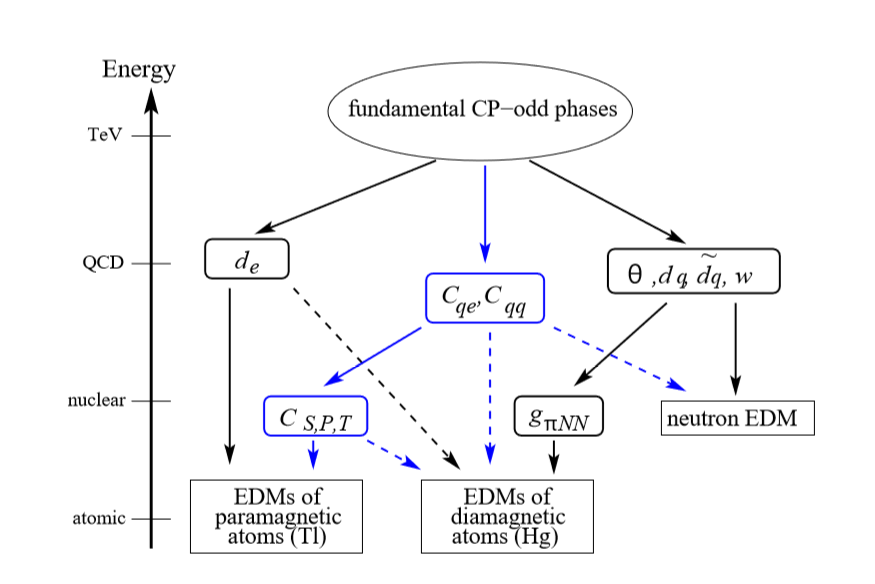
\includegraphics[width=0.8
	\textwidth]{OverviewPicture.png}
	\caption { A schematic plot of the scales between CP-odd sources from the physics review by Pospelov and Ritz \cite{Pospelov2005} shows how new physics from the TeV scale interactions feeds into operators and parameters at the scales of \gls{qcd}, nuclear physics and atomic energy scales, the solid lines represent the important contributions that lead directly from one level to another.}
		\label{fig:EDMsource}
\end{figure}

Fundamental theories set the scale of an EDM, or are have parameters that set the strength of CP-odd process that give rise to the EDM. Fig. \ref{fig:EDMsource} shows the contributions to atomic \gls{edm} from the atomic, nucleon, and QCD energy levels being fed by fundamental CP-odd phases. At the atomic level the atom can be either paramagnetic (spin-1/2 electron unpaired) or diamagnetic (spin-0 pair of electrons). 

The paramagnetic atoms directly couple to the electron  \gls{edm} $d_e$, with connections from nuclear effects $C_{S,P,T}$. Here $C_{S,P,T}$ are quark-electron coupling strength $C_{qe}$ for \gls{qcd} expressed as an effective field theorem at the nuclear scale. For diamagnetic atoms the picture is more complicated, and in addition to contributions to their \gls{edm} that are the same as in the paramagnetic case, they have contributions from $g_{\pi NN}$ coupling constant between pions and the nucleons in the nucleus, the quark EDM $d_q$, and the strong-CP phase $\theta$. 

The CP-odd parameters and interaction give rise to the EDMs of these observables at the atomic level. Specifically, looking at the effective field theory Lagrangian at the nuclear scale level: there are the direct contributions from particles such as the neutrons, proton and the electron EDMs; the CP-violating electron-nucleon and nucleon-nucleon interactions; and the CP-odd pion-nucleon interactions. The second term can be though of as the nucleon induced EDM. The Lagrangian is given by

\begin{equation}
    \begin{split}
        \mathcal{L}^{\textrm{nuclear}}_{eff} =  \mathcal{L}_{\textrm{edm}} (d_e, \, d_n, & \, d_p)+  \mathcal{L}_{\pi \textrm{NN}}(\bar{g}^{(0)}_{\pi \textrm{NN}}, \, \bar{g}^{(1)}_{\pi \textrm{NN}}, \, \bar{g}^{(2)}_{\pi \textrm{NN}} )\\+ 
        & \mathcal{L}_{eN}(C_{\textrm{S}}, \, C_{\textrm{P}}, \, C_{\textrm{T}}).
    \end{split}
\end{equation}
%with the specific therms given by:
%\begin{equation}\label{eq:Ledm}
%    \mathcal{L}_{\textrm{edm}}=-\frac{i}{2} \sum_{i=e,p,n}d_i\bar{\psi_i}(F\sigma)\gamma_5 \psi,
%\end{equation}
%
%\begin{equation}\label{eq:Lpnn}
%    \mathcal{L}_{\pi \textrm{NN}}=
%    \bar{g}^{(0)}_{\pi \textrm{NN}} \bar{\textrm{N}} \tau^a \textrm{N}\pi^a+\bar{g}^{(1)}_{\pi \textrm{NN}} \bar{\textrm{N}}\textrm{N}\pi^0
%    +
%    \bar{g}^{(2)}_{\pi \textrm{NN}}( \bar{\textrm{N}} \tau^a \textrm{N} \pi^a-\bar{\textrm{N}}\tau^3\textrm{N}\pi^0),
%\end{equation}%
%
%\begin{equation}\label{eq:Len}
%    \begin{aligned}
%           \mathcal{L}_{e\textrm{N}}={}&
%    C^{(0)}_{\textrm{S}} \bar{e}i\gamma_5 e  \bar{\textrm{N}}\textrm{N}+ C^{(0)}_{\textrm{P}} \bar{e} e  \bar{\textrm{N}} i\gamma_5\textrm{N}
%    +   C^{(0)}_{\textrm{T}}\epsilon_{\mu \nu \alpha \beta} \bar{e} \sigma^{\mu \nu} e  \bar{\textrm{N}} \sigma^{\alpha \beta}\textrm{N} \\
%    &+ C^{(1)}_{\textrm{S}} \bar{e}i\gamma_5 e  \bar{\textrm{N}}\tau^3 \textrm{N}
%    + C^{(1)}_{\textrm{P}} \bar{e} e  \bar{\textrm{N}} i\gamma_5\tau^3 \textrm{N}
%    + C^{(1)}_{\textrm{T}}\epsilon_{\mu \nu \alpha \beta} \bar{e} \sigma^{\mu \nu} e  \bar{\textrm{N}} \sigma^{\alpha \beta}\tau^3 \textrm{N}.
%    \end{aligned}
%\end{equation}
Succinctly, the Lagrangian $\mathcal{L}$ can be expressed as a set of interaction coefficients $\alpha_i$ of the interactions defined by CP-odd interaction operators $\mathcal{O}^{CP}_i$, where the subscript $i$ sums over all of the CP-odd interactions. The succinct form of the Langrangian is 
\begin{equation}
    \mathcal{L} = \sum_i \alpha_i \mathcal{O}^{CP}_i.
\end{equation}
 At the nuclear scale, the coefficients of the Lagrangian $\alpha$ have a complicated dependence on the observable atomic EDM. The dependence of the strength of interaction is a many body nuclear problem. 
 
 It is important to note that in addition to the electron EDM, $d_e$, the quark-quark and quark electron interactions $C_{qq}$, and $C_{eq}$ play an important role in determining the interactions that generate the EDM of paramagnetic atoms. The atoms of $^{129}$Xe or $^{199}$Hg are diamagnetic, but it is still important to discuss the physics for a paramagnetic atom. 
 
 The paramagnetic atom acquires an EDM from an unpaired relativistic electron that in the valance shell. The EDM grows stronger with increasing atomic number since the orbitals have higher atomic radius. The strength of EDM of paramagnetic atom is given by
\begin{equation}
    d_{para}(d_e) \sim 10 \frac{Z^3 \alpha^2}{J(J+1/2)(J+1)^2} d_e,
\end{equation}
where $Z$ is the atomic number, $J$ is the angular momentum quantum number, and $\alpha$ is the fine structure constant.

For diamagnetic atoms, the contributions to the  EDM are from a collection of relevant parameters, including the Schiff moment contribution from the nucleus
\begin{equation}
    d_{dia}=d_{dia}(S[\bar{g}_{\pi N N },d_N],C_S,C_p,C_T,d_e).
\end{equation}
Schiff's theorem states that a point-like nucleus in a non-relativistic cloud of electrons would experience negligible nuclear EDM due to the screening of the nuclear EDM from the electrons. A Schiff moment is the name given to the EDM moment that violates Schiff's Theorem. In the nucleus P-odd and T-odd nucleon-nucleon interactions $g_{\pi N N}$ lead to CP-violation. Finite sized nuclei violate Schiff's theorem because the electrons can be relativistic, and the nucleus may not be symmetric \cite{Flambaum, Sushkov}.

Typical beyond standard model theories predict a larger EDM than predicted in the SM. So far only limits on EDM have been placed, leading to upper bounds on particle \gls{edm}s, which can be interpreted as limits on the parameters of the beyond standard model physics.
%Why focus on Diamagnetic and neutron EDM

\chapter{EDM measurment methods}

This chapter provides a brief summary of the theory involved in the neutron, $^{129}$Xe and $^{199}$Hg \gls{edm} measurements. In particular it will review the magnetic moment interactions, techniques used to measure polarization and methods of polarizing the sources. 

\section{Magnetic moments and polarization}

The magnetic moment is a fundamental property of quarks and the electron. The spin components of quarks follow sum rules that dictate the spin axis $\vec{J}$ of the resulting particle (meson, bayron, hadron, etc.). The magnetic moment itself if defined as
\begin{equation}
    \vec{\mu}=\gamma \hbar \vec{J}.
\end{equation}
Here  $\gamma$ is the gyromagnetic ratio of the particle which relates the frequency of oscillation of the spin vector about a magnetic field due to its magnetic moment, and $\hbar = 1.054571\times 10^{−34}$ J$\cdot$s is Planck's constant.  In the presence of a magnetic field with a magnitude $B_0$ the magnetic moment precesses about the magnetic field with a frequency, $\omega$, given by
\begin{equation} \label{eq:bfrequency}
    \omega = \gamma B_0 .
\end{equation}
The action of the magnetic field on the Hamiltonian induces an energy splitting known as Zeeman splitting. Using only the magnetic component of Eq. \ref{eq:hamiltonian}, and solving for a static magnetic field, $B_0$, the resulting eigenvalue equation is related to the direction of the spin vector, and the magnetic field. The resulting energy splitting is: 
\begin{equation}
    E = -\mu B_0 \frac{m_J}{J}, %\sim 60 \; \textrm{neV/T},
\end{equation}
where $m_J = (-J,\, -J+1,\, \ldots,\, J-1,\, J ) $ is the spin quantum number corresponding to the allowable projections of spin onto the magnetic moment axis. In a spin $J=1/2$ system the allowable values of $m_J=\pm 1/2$ correspond to the energy splitting $E=\mp \mu B_0$. 

There is an analogous splitting in energy due to an EDM in an electric field, called the Stark effect. The combination of Zeeman splitting and Stark splitting are what allow you to measure the frequency difference from an EDM. The energy differences between the split states with aligned magnetic and electric fields ($B_0$ and $E_0$) are given by
\begin{align}
    \Delta E(B\uparrow,E\uparrow) = \hbar \Delta \omega_{\parallel} =& 2\mu B_0 + 2d  E_0 \,\textrm{and}\\
    \Delta E(B\uparrow,E\downarrow)= \hbar \Delta \omega_{\nparallel} =& 2\mu B_0 -2 d E_0.
\end{align}
Solving these two equations the \gls{edm} $d$ is given by
\begin{equation}
    d=\frac{\hbar(\omega_\parallel - \omega_\nparallel)}{4E_0},
\end{equation}
which means that the EDM is measured by the difference in the frequency of oscillations when the magnetic field and electric field are parallel to when they are antiparallel.

Particle polarization, $P$, is defined as the fractional population difference between the positive high field seeking state $m_J=+1/2$ and the low field seeking state $m_J=-1/2$ by
\begin{equation}
    P  =\frac{N_+-N_-}{N_+ +N_-},
\end{equation}
where $N_+$ and $N_-$ are number of particles with spin state of $m_J = +1/2$ and $-1/2$ respectively. Highly polarized systems will have one population of the spin states much greater than that of the other state.  


\section{UCN EDM}

\subsection{Ultracold neutron polarization process}
Neutrons decay via the weak force with a half-life of 881 s, or about 10 minutes when not bound in an atom. In order to have a source of free neutrons for any non-bound neutron experiment they must be liberated from the nucleus. Once liberated neutrons that are free from the nucleus are slowed down in progressively colder materials. The UCNs are slowed through kinematic reactions with cold moderators and transfer energy to the cold moderators until they reach the energy necessary to be classified as an \gls{ucn} \cite{Golub}.  

\Gls{ucn} interact with all of the forces of the \gls{sm}. They interact via the strong force in Fermi interactions with the walls of all containers they are stored in $\leq 300$ neV, the electromagnetic field interactions with magnetic moment, and the weak force is cause of neutron decays. Additionally, \gls{ucn} feel a gravitation potential of V $\sim 100$ neV/m. The magnetic field interactions are how the UCN are polarized via
\begin{equation}
    V = \mp \mu B_P \; \; \; \sim \;\mp60 \,\textrm{neV/T},
\end{equation}
where a strong enough polarizing magnetic field $B_P$, can to block UCN of low field seeking spin states $(-\mu B_P)$, and allow the other spin state $(+\mu B_P)$ to propagate through for the neutron spins $m_J=+1/2$ and $m_J=-1/2$ respectively.  The resulting neutron beam is polarized up to an energy range set by the magnitude of the magnetic field for one of the spin states. 

\subsection{Nuclear magnetic resonance pulses and the Ramsey sequence}

In the rotating frame of reference, $S'$, of the oscillating magnetic moment rotating about the z-axis with frequency at the Larmor frequency $\omega_0$, the static coordinates in the static frame $S$ transform according to

\begin{equation}
    \begin{split}
        x' =& x \cos{ \omega_0 t} - y \sin{\omega_0 t}\\
        y' =& x \sin{\omega_0 t} + y \cos{\omega_0 t}\\
        z' =& z.
    \end{split}
\end{equation}

In the frame of reference $S'$ the spins act as if the polarization vector is held in place, and no longer sees the static  magnetic holding field $B_0$ at all. If the system is subjected to an oscillating magnetic field $B_1(t)=\cos{(\omega)}$ perpendicular to $z'$ at the same frequency as that of $\omega_0$ , the magnetic spins will evolve in the rotating frame as they were only subjected to a magnetic field along a the $x'$-direction. The spins will now start to precess about that new rotating vector  with a new frequency $\omega_1 = \gamma B_1$. The amount of rotation that the polarization vector undergoes in frame $S'$ can be set by limiting the time $B_1$ is on, defining a pulse length in time. A full $2\pi$ rotation would have a pulse length of $t_1$. To undergo a $\pi/2$ rotation, the particle of interest is subjected to an pulse at a time of $t_{\pi/2}$ defined by

\begin{equation}
    t_{\pi_{1/2}}=\frac{1}{4}t_1=\frac{\pi}{2 \gamma B_1}
\end{equation}


\begin{figure} [htbp]
	\center
	\subfigure[]{
	    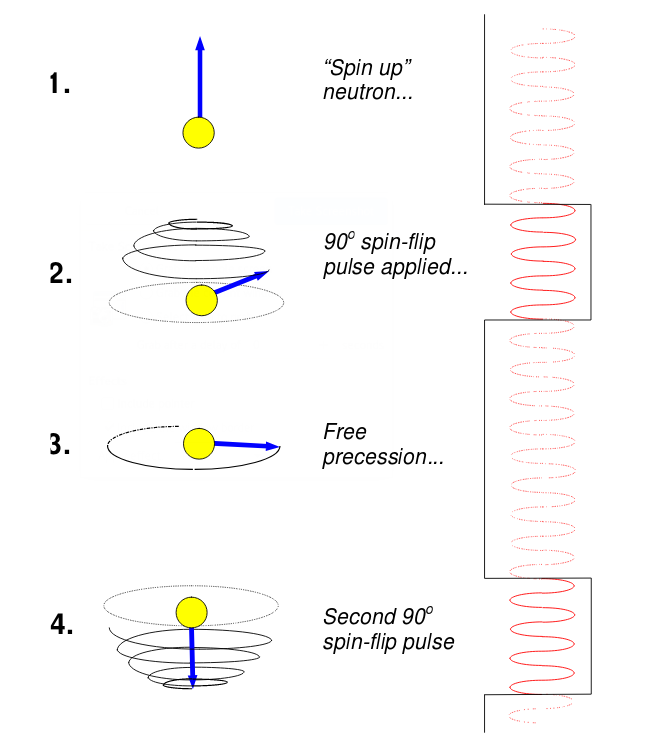
\includegraphics[width=.35\textwidth]{RamseySequence.png}}
	\hfill
	\subfigure[]{
	    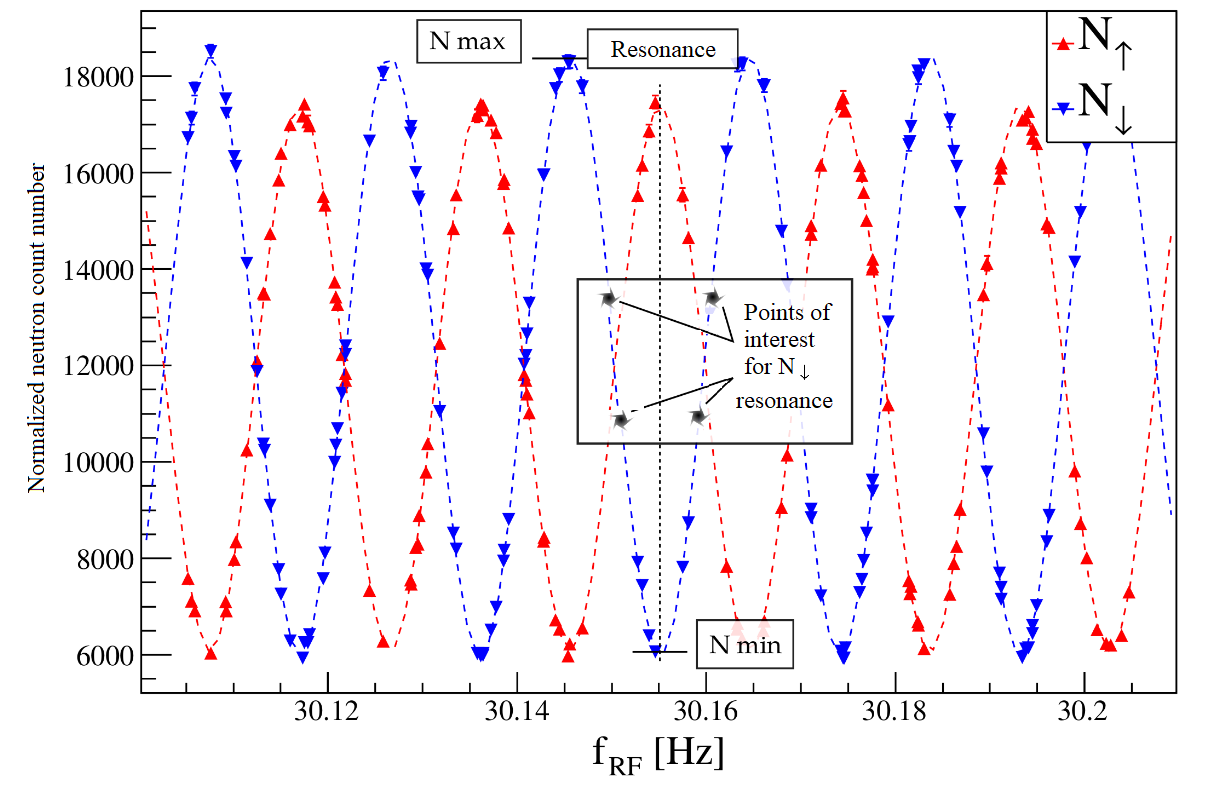
\includegraphics[width=.6\textwidth]{RamseyFringe.png}}
	\caption {Ramsey technique, shown left (a), is used measure oscillating frequency and starts with (1) polarization along one direction, (2) then a cosine pulse is applied to tilt the spins, (3) then a spins are allowed to free process (4) an identical in-phase RF-pulse is applied to tilt the spins again. Figure from Harris \cite{Harris2007}. The Ramsey fringe, shown right (b), is a direct measure of spin states $N_{\uparrow, \downarrow}$ sweeping the ocilating fields frequency $\omega_1$. The central resonance of the Ramsey field can be determined by the 4 off resonance points of interest. Figure adapted from Victor H\'elaine's thesis \cite{Helaine2014}. }
		\label{fig:Ramsey}
\end{figure}


The Ramsey method can be used to determine the frequency of oscillation \cite{Ramsey1980}. First, a polarized particle is placed in a static magnetic field. The system is subject to a oscillating magnetic filed pulse with frequency $\omega_{RF}$ for a time $\tau$, allowed a period of free procession $T$, and then subject to another pulse that is coherent with the original one as show in Fig. \ref{fig:Ramsey}a. The term RF is borrowed form nuclear magnetic resonance to denote a $B_1$ transverse pulse, and not to denote its frequency which is typically tens of Hertz. Doing a Ramsey sequence over another frequency $\omega_{RF} \ne \omega_0$ produces incomplete slip flipping when off resonance. The probability of the state to be in its original system is given by
\begin{equation}
    P=1-4\sin^2{\theta} \sin^2 {\frac{a\tau}{2}} \Big[\cos{\frac{\lambda T}{2}} \cos{\frac{a \tau}{2}}-\cos{\theta}\sin{\frac{\lambda T}{2}} \sin{\frac{a\tau}{2}}\Big]^2,
\end{equation}
where
\begin{equation*}
    \begin{split}
         \cos{\theta} = -\omega_{RF}/a, \;\;\;\;\;\;\; \sin{\theta}= & 2b/a, \;\;\;\;\;\;\;  a = \sqrt{\omega_{RF}^2+(2b)^2},\\
         b = \omega_0 \frac{B_1}{B_0}& , \;\;\;\;\;\;\; \lambda =\omega_0-\omega_{RF}.
    \end{split}
\end{equation*}
The population distribution function $P(\omega_{RF})$ describes a Ramsey fringe and is shown in Fig. \ref{fig:Ramsey}b in blue.

\subsection{The neutron electric dipole moment experiment}

The world's leading \gls{nedm} measurement was conducted at \gls{ill}, Grenoble using an atomic Mercury comagnetometer to achieve an upper limit on the magnitude of the \gls{nedm}  ${} <\; 3.0 \times 10^{-26}$ \textit{e} cm (90\% CL) \cite{Pendlebury2015, Baker2006}.

\begin{figure} [htbp]
	\center{
		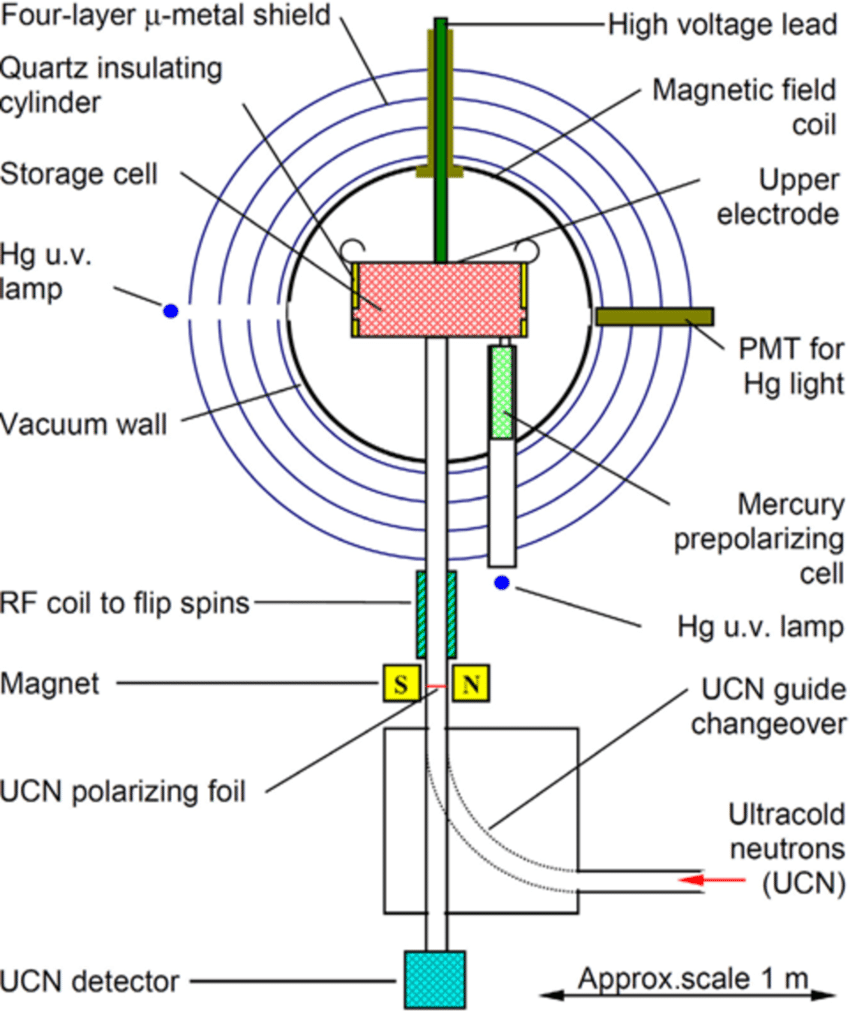
\includegraphics[width=0.45\textwidth]{nEDM.png}
	}
	\caption {Schematic diagram for the neutron electric dipole moment experiment at \gls{ill}, Grenoble \cite{Baker2014}. \gls{ucn} enter from a source via a \gls{ucn} guide located at the bottom right travel through a polarization foil on their way to the storage cell and remain aligned to a global B-field. Once there a static E-field is applied parallel or anti-parallel to the B-field, while a transverse RF field produced the pulse necessarily for the Ramsey method of frequency separation.}
		\label{fig:nedm}
\end{figure}

The \gls{nedm} measurement is performed inside a four layer $\mu$-metal shield. The magnetic shield is required to decrease the magnitude and gradient background B-fields that the neutrons see to a level of less than 1 nT/m. By lower the B-field gradient false \gls{edm}s that can mimic a EDM are reduced.

\gls{ucn}s from the source are transported into the set up, where they first interact with a \gls{ucn} polarizing foil.  The polarized \gls{ucn} travel into the storage cell, which contains a cohabiting mercury gas. An ultraviolet mercury lamp below the UCN cell is used to polarize the Hg atoms before \gls{ucn} filling. Once the pre-polarizing is completed via optical pumping, the Hg gas vapor is leaked into the storage cell to act as a comagnetometer. The mercury co-magnetometer is used to correct the data from false \gls{edm}s due to any systematic effects caused by magnetic field gradients.

Once in the cell, the UCN undergo a Ramsey sequence as shown in Fig. \ref{fig:Ramsey}. The polarization of the UCN is determined by emptying the cell through an analyzer foil into a UCN detector below.  By measuring UCN after different RF frequencies are used, points on the Ramsey fringe curve are used to determine the resonant frequency. The experimental data are taken at four frequencies, two on either side of the resonance frequency, at the maximum slope on either side of the Ramsey central fringe to get the best fit of the Ramsey central fringe. The signature of a neutron EDM is a shift in the frequency in of the central fringe under reversal of the E field. Using the polarizer / analyzer foil only a particular polarization state of \gls{ucn} are measured.  An RF coil in an adiabatic fast passage spin flipper is used to flip the spins allowing the other polarization state to be measured. The neutrons' final polarization is $\alpha$. The frequency is determined by the Ramsey technique, and $d_n$ with statistical uncertainty $\sigma_d$ is given by:

\begin{equation}
    \begin{split}
        d_n = & d_n \pm \sigma_d \\
        d_n = &\frac{\hbar(\omega_\nparallel - \omega_\parallel)}{4E}\\
        \sigma_d \approx & \frac{\hbar}{2 \alpha E T \sqrt{N}}
    \end{split}
\end{equation}

where $E$ is the magnitude of the electric field, $\alpha$ is the polarization of the neutrons, $T$ is the free precession time of the Ramsey sequence, $N$ is the total number of counts, $\omega_\parallel$ is the frequency of precession determined from the Ramsey technique when the B and E field are parallel $B\uparrow E\uparrow$, and  $\omega_\nparallel$ is the frequency of procession determined from the Ramsey technique when the B and E field are anti-parallel $B\uparrow E\downarrow$.

\section{Xenon EDM}

\subsection{Xenon polarization process and polarization detection}\label{sec:SEOP}
\Gls{seop} is used in the production of hyper-polarized xenon and helium noble gas used in the $^{129}$Xe \gls{edm} experiment. \gls{seop} is a two stage process that consists of optical pumping followed by a spin exchange interaction. 

Optical pumping of Rb is carried out with circularly polarized light $\sigma^+$ from a 794.7~nm laser array that excites a transition in the valence electron of the Rb atom from a $^2\textrm{S}_{1/2}$ into a higher energy level $^2\textrm{P}_{1/2}$ in the presence of a magnetic field. The magnetic field is necessary to split the degenerate spin states into non-degenerate Zeeman states. The change of momentum of $\Delta m_f=+1$ induced from the laser light and the selection rules of $\Delta m_F = -1,0,+1$ ensures that the excitations disproportionately build up to higher angular momentum states as the atoms are pumped continuously. With strong enough laser power the maximal angular momentum state $F=+3, \; m_F =3$ is populated fully. An energy and spin state diagram of $^{85}$Rb showing allowable states that optical pumping transitions can go to are shown in Fig. \ref{fig:Rb-levels}.

\begin{figure}[h!]
    \center
    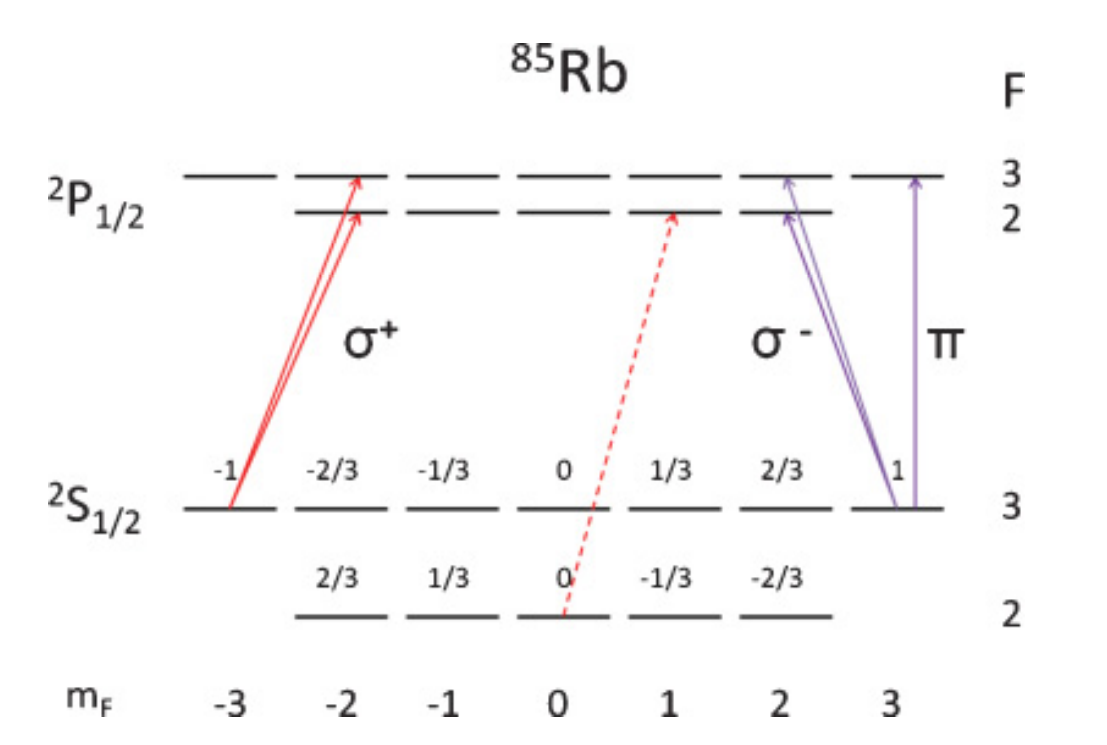
\includegraphics[width=.55\textwidth]{85Rb-levels.png}
    \caption{The magnetic levels of a $^{85}$Rb atom for the $^2$S$_{1/2}$ and the $^2$P$_{1/2}$ transitions. $\sigma^\pm$ is circularly polarized light and $\pi$ is linearly polarized light. The solid arrows indicate selection rules that the light can follow $\sigma\pm \xrightarrow{} \Delta m_F = \pm 1$ amd $\pi = \Delta m_F = 0$.  The solid red light is the laser light transition with circular polarization $\sigma^+$ that we are interested in. Figure taken from Norrgard et al.  \cite{Norrgard2010}}
    \label{fig:Rb-levels}
\end{figure}

The second part of SEOP is the spin exchange process. Spin exchange of the polarized Rb atom with Xe is mediated by an inert buffer gas, N$_2$. The spin of the Rb atom is transferred to Xe via contact interactions in weakly bound states. The states evolve according to the Hamiltonian 
\begin{equation}
    H = A \vec{I}\cdot \vec{S}+\gamma \vec{N}\cdot \vec{S}+\alpha \vec{K}\cdot \vec{S},
\end{equation}
where $A$, $\gamma$, and $\alpha$ are the interactions strengths, $\vec{S}$ is the electron spin of the Rb atom, $\vec{I}$ is the atomic spin of the Rb atom, $\vec{N}$ is angular momentum of a Xe-Rb weakly bound system, and $\vec{K}$ is the atomic spin of the Xe \cite{Happer1984}. The last term dominates the spin exchange process leading to an exchange of spin of the Xe and Rb. An identical process happens with He as well, polarizing it in the same SEOP cell. 

The Xe and He polarization systems are called masers from the ammonia maser device, which operates at a frequency in the microwave range. The first maser device was an atomic clock with very stable atomic oscillations. A maser consists of a polarization selector, which in the case of Xe is a SEOP polarizer. The polarized atoms in the maser are then supplied to a cell where a pickup coil surrounds it. The atoms in the maser experiences a loss in polarization due to the radiative damping from the pickup coil. An important feature of the maser is that the pick up coil is tuned to the resonant frequency of the oscillations. There is a feed back loop from the signal that changes the magnetic field causing the Zeeman levels to match the frequency of the pick up coil.  This results in the optimal signal stability, and reaches equilibrium in the rotating frame at the Larmor frequency $\omega_z$.  In equilibrium, the rotating polarization vectors are given by
\begin{equation}
    \begin{split}
        P^{eq}_Z  =& P_0 \frac{\tau_{RD}}{T_2} \frac{\omega_0}{\omega_z \cos^2{(\delta)}} \; \; \textrm{and}\\        
        P^{eq}_X =& \sqrt{(P_0 \tau_{RD}) \frac{\omega_0}{\omega_z \cos^2{(\delta)} }P_0 \bigg( \frac{1}{T_1}+G_m\bigg) \bigg(1-\frac{\tau_{RD}}{T_2} \frac{\omega_0}{\omega_z \cos^2{(\delta)} } \bigg)},
    \end{split}
\end{equation}
where the resonant frequency of the pick-up coil is given by $\omega_0$, the detected frequency is given by $\omega_z$, $P_0$ is the polarization if there was no coil, $G_m$ is the influx of polarization from the SEOP cell, $T_1$ is the return to polarization decay term, and $T_2$ is the transverse decay term.   

The pick up coil's resonance $\omega_0$ is tuned to match the oscillations of the Xe in the maser. This eliminates the phase shift $\delta$ between the pick-up coil's resonance and the Larmor resonance. The inset of Fig. \ref{fig:Maser} shows the Bloch vector $\textbf{M}$, a constant vector in the rotating from. The radiative damping term from the pick-up coils tip the polarization vector, causing a polarization build up in the transverse direction. The resonant equilibrium oscillations of the atomic species are given by
\begin{equation}
    \omega_z = \gamma B_0 - \frac{1}{T_2} \frac{\sin(\delta)}{\cos{(\delta)}}.\label{eq:maserOmega}
\end{equation}

Near equilibrium oscillations of the vector sum signal of the Larmor precession can easily be induced ontop of the equilibrium signal by external perturbations. Such temperature and vibrational fluctuations can create a long lasting signal that is not analytically solvable. The long lasting signal can be numerically solved, and the data can be fit to a decaying sinusoidal function as a numerical approximation via
\begin{equation}
    \delta P_Z\sim \sin{(\omega t + \phi)}e^{\Gamma t},\label{eq:maserPerturbedOmega}
\end{equation}
where $\omega$ is the frequency of the new perturbative oscillations in the rotating frame, with a phase of $\phi$, and a decay constant of $\Gamma$. The decaying oscillations are related to the resonant frequency by
\begin{equation}
    \omega \approx \sqrt{2} \frac{P^{eq}_X}{P_0 \tau_{RD}}.
\end{equation}
The decaying sinusoid is fit, and the frequency that is found is used to calculate the resonant frequency of the Xe and He. 
%
%Small changes from on-resonance will make the oscillating polarization behave  like a driven Bloch equation with small perturbations given by:
%
%\begin{equation}%give the 
%    \begin{split}
%       \delta \dot{P}_x =& \frac{P^{eq}_x}{P_o\tau_{rd} } \delta P_z,\\
%        \delta \dot{P}_z =& FG_m\delta  P_z -\frac{2P^{eq}_x}{P_o\tau_{rd}}\delta P_z- \Big(G_m+\frac{1}{T_1}\Big) \delta P_z,\\
%        \delta \dot{P}_P =& FG_p\delta  P_z - \Big(\gamma_{se}+G_m+\frac{1}{T_1} \Big)\delta P_z.
%    \end{split}
%\end{equation}
%
%Here the polarization perturbation is given by $\delta P_i$ for the x, z and transverse P directions, $G_m$ accounts for longitudinal transport of polarization into the cell, $T_1$ is the NMR decay constant of the longitudinal polarization, $P_0$  is the initial polarization, and $G_P$  is depolarization from tr into the cell \cite{Rosenberry2000}. The  constant $F$ is related to transfer tube losses. These coupled equations does not have an analytical solution, but neglecting transport effects from $P_P$ then it becomes a decaying sine wave equation with angular frequency
%
%\begin{equation}
%   \omega \approx \sqrt{2} \frac{P^{eq}_x}{P_o\tau_{rd}}.
%\end{equation}

\subsection{Xe Maser EDM Experiment}

The world's leading measurement of the \gls{edm} of $^{129}$Xe set the upper bound of the to be $< 6.6 \times 10^{-27}$ \textit{e} cm (95\% CL) \cite{Rosenberry2001}. This experiment's measurement of the EDM of $^{129}$Xe is based on the frequency difference of polarized Xe and that of a $^3$He oscillator. The experimental cell contains the Xe and He atoms sealed off after nitrogen gas, N$_2$, is added. Here N$_2$ serves as a buffer gas. 

\begin{figure} [h!]
	\center
		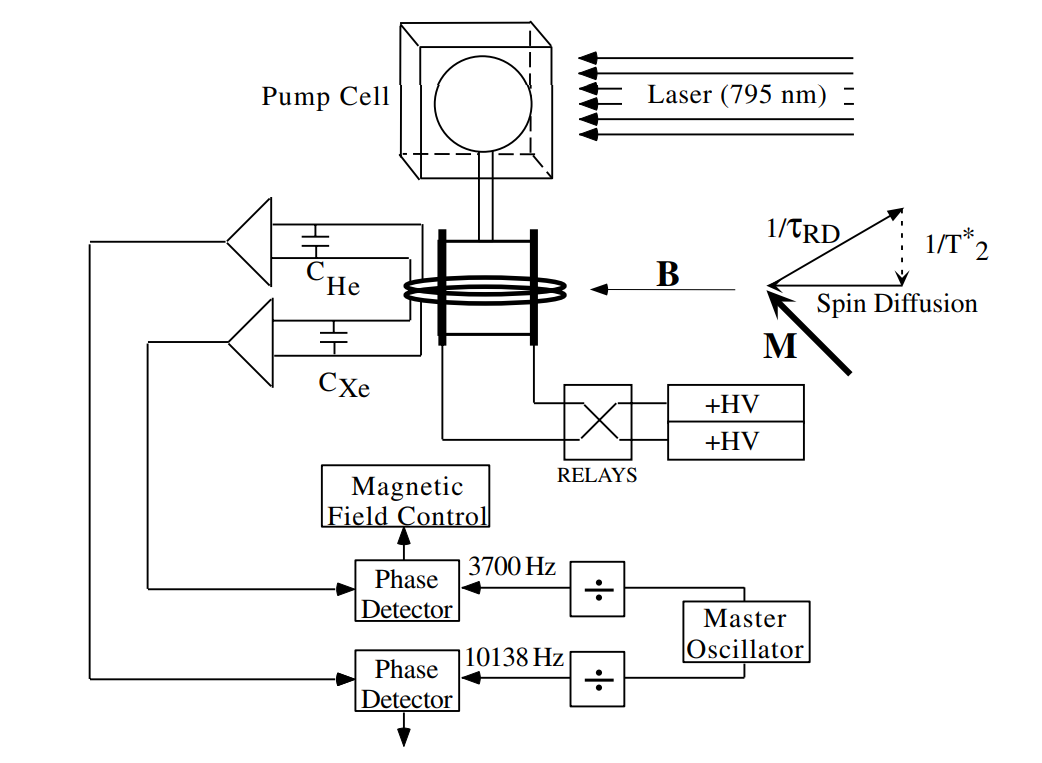
\includegraphics[width=0.7\textwidth]{MaserXeExperiment.png}
	\caption { Schematic diagram for the $^{129}$Xe maser experiment using a $^3$He maser comagnetometer from Rosenberry and Chuup \cite{Rosenberry2001}. The Bloch vector \textbf{M} and its contributing vectors is inset in the diagram. }
		\label{fig:Maser}
\end{figure}

A Rb laser array is used to pump the Xe and He into polarized states via \gls{seop} of Rd vapour inside a pump cell. The polarized states continuously diffuse into the masing cell where there are electric and magnetic fields. The frequency of oscillation is determined via masing action in a pick-up coil wound transverse to the $B_0$ holding field. $^3$He acts as comagnetometer measuring same magnetic field that the $^{129}$Xe sees by sampling the same cell simultaneously.

The Bloch vector \textbf{M} in Fig.~\ref{fig:Maser} illustrates the three contributing effects to a stationary state signal: the spin diffusion from the pump cell to the maser cell provides a net alignment to the magnetic field; $\tau_{rd}$ is the radiative dampening term and is associated with polarization lost in the pick up coils surrounding the cell due to masing; and $T_2^*$ is a combination of the  spin loss terms containing the spin relaxation $T_2$ term, and any other spin loss mechanisms. The spin loss mechanisms include: polarized atomic species diffusing back into the pump cell; losses of polarization due to magnetic field gradients; and wall losses. 

A master oscillator is detuned 25 mHz below the resonant Larmor frequency of $^{129}$Xe which is given by $\omega = \gamma_{\textrm{Xe}} B_0$. The signal from the pickup coil is multiplied to the master oscillator signal and the resulting beat signal is locked via a two phase detector lock-in amplifier. The frequency of the $^{129}$Xe maser corrects the magnetic field via a control loop to maintain a stead-state precession signal. Any change in frequency of the Xe signal will result in a 2.8 times greater change in the $^3$He maser frequency due to the differences in their gyromagnetic ratio $\gamma_{\textrm{He}}/\gamma_{\textrm{Xe}}$. The enhances sensitivity to the magnetic field means that the He maser will experience greater systematic caused by and magnetic field gradient and can be used as a co-magnetometer.

An electric field E is provided by a \gls{hv} that is changed in a controlled manner between each measurement and will determine the resulting output frequency change strength due to any potential \gls{edm} measured by difference in the maser frequency. The varying electric field used are $E = \pm 3.6$ kV/cm and 0, which are changed in sequence. Typically the electric field sequence used in the measurement is $( \ldots + - + - 0 - + - + 0 + - + - 0 \ldots )$, but the order was changed occasionally to test systematic effects. In order to compute the EDM, the frequency is corrected from the higher sensitivity $^3$He comagnetometer, and each run is calculated from a set of four measurements, which are assumed to be correlated, using consecutive $E$ scans defined by:

\begin{equation}
    \omega_{i+n}-\omega_{i}=\frac{2d}{\hbar}(E_{i+n}-E_i)+n\Delta+n^2\Delta^2,
\end{equation}

where the subscript $i =1, \, 2, \, \ldots, \, N-3$  denotes the run number in $N$ runs,  $n=1,2$ or $3$ denotes the consecutive scan number, $\omega_i$ is the corrected frequency, and $d$ is the EDM measured for that particular run. The $\Delta$ term denotes possible linear and quadratic drifts that are included from a quadratic fit that corrects for magnetic fields fluctuations. The variance in the fit parameters determines the statistical uncertainty of the change $\Delta \omega$.

\section{Mercury EDM}

\subsection{Mercury polarization and polarization detection process}

Synchronous optical pumping is carried out in an identical manner to the optical pumping described in Sec. \ref{sec:SEOP} but the pump beam is chopped at the Larmor frequency of the atom. The Hg atoms are pumped with a circularly polarized laser light at 253.7 nm, corresponding to the excitation from the state $F = 1/2$ to $F = 1/2$ transition from the $^1\textrm{S}_0$ to the $^3\textrm{P}_1$ state as shown in Fig. \ref{fig:HgLevels}. A rotating optical chopper is operated synchronously at the Larmor precession frequency, causing the pump light to impinge on the Hg atoms in synchronous bursts. The synchronized optical pumping of the atoms polarizes the atoms transverse to the magnetic filed. The optical pumping is switched between the synchronous mode where the laser produces a coherent pi pulse and a continuous non-pulsed mode, and back again, to achieve a high level of coherent transverse polarization.

\begin{figure}[htbp]
    \center
    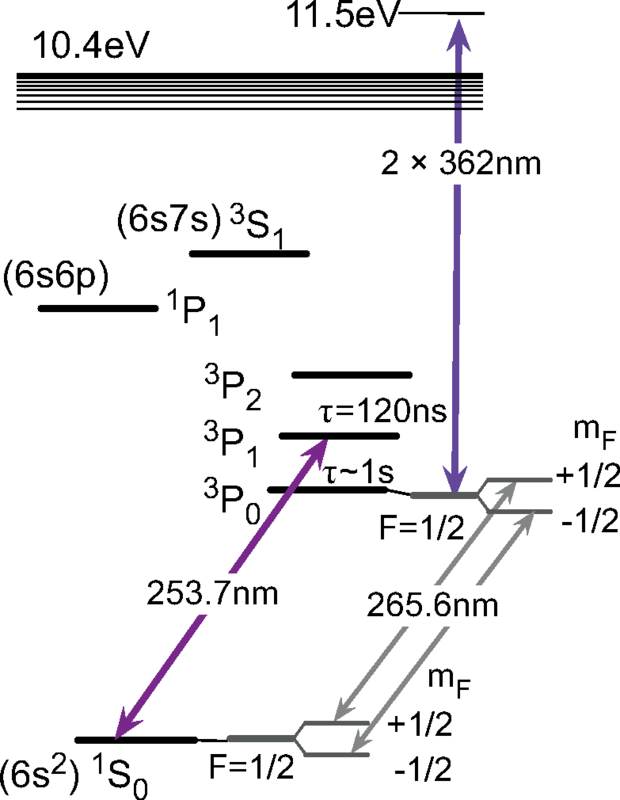
\includegraphics[width=0.3
    \textwidth]{199Hglevels.png}
    \caption{The excited states of $^{199}Hg$ electron transition rules. Figure from McFerran et al. \cite{McFerran2014}}
    \label{fig:HgLevels}
\end{figure}

\begin{figure}[htbp]
    \center
    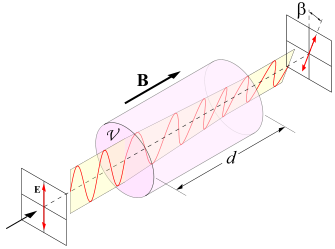
\includegraphics[width=.4\textwidth]{Faraday.png}
    \caption{Faraday rotation of the linearly polarized light by an angle $\beta$ when the light traverses a medium a distance $d$. The size of the angle is related to a coefficient $\mathcal{V}$, which is the Verdet constant. The constnat $\mathcal{V}$ depends on the dielectric properties of the material. For a changing electron density this is not constant but time dependent. }
    \label{fig:Faraday}
\end{figure}

The Faraday rotation signal is used to determine the oscillation frequency of $^{199}$Hg. Faraday rotation is a magnetic optical process that rotates the linear polarization of light as it traverses a medium. In a dielectric material the equation of rotation in Fig \ref{fig:Faraday} is given by

\begin{equation}
    \beta = \mathcal{V}Bd,
\end{equation}
where $\beata$ is the Faraday rotation angle,  $B$ is the magnetic field parallel with the path of travel, $d$ is the interaction length of the dielectric material and $\mathcal{V}$ is the Verdet constant. The medium's magnetic moment and external magnetic field causes the polarization of the light to rotate if the field is parallel to the propagation path. In fact, this rotation angle $\beta$ is be determined by the path parallel to the magnetic field $\vec{B_\parallel}$, the medium dependant constant for the density of electrons $n(z)$, and interaction length $d$ by

\begin{equation}
    \beta =  \frac{e^3}{2\epsilon_0m^2_ec}\frac{1}{\omega}\int_z^{z+d} n(z)B_\parallel (z)dz
\end{equation}

If the component of the magnetic field parallel to the optical path has a characteristic time dependence ${B_\parallel}(t,z)$ the angle of rotation will also oscillate as a function of time $\beta(t)$. The probe beam defines our axis of interest. Precessing Hg atoms create a rotating magnetic field perpendicular to the atoms polarization vector. The probe beam is set up perpendicular to the holding magnetic field and is used to pick this sinusoidal decaying signal of the Hg atoms up via Faraday rotation. The polarization decays away exponentially with the transverse polarization decay time of $T_2^\star$.

After pumping, the laser is detuned, the intensity is attenuated through a density filter, and switched to linearly polarized light so that the frequency of the laser lies halfway between the excited states  $F=1/2$ and $F=3/2$. This detuned pump laser will now act as a probe laser to sample the atoms' phase by Faraday rotation. The measured rotation angle
\begin{equation}
    \theta(t)=\theta_0 \sin{(\omega t + \phi)}e^{-t/\tau},
\end{equation}\label{eq:faraday} 
oscillates with the frequency $\omega$ of the rotating magnetic moment of the Hg atoms distorted by the probe beam. The unperturbed frequency is then extracted from the phase difference of two short probe beams separated by a dark period $\Delta t^D_{AB}$. The two probe periods are labelled probe period A and probe period B. The time $t=0$ is taken at the end of the probe A in the fit of phase $\phi^D_{A}$. The fit is used to extract the phase difference of the signal at the end of a short probe beam $\phi_A^D$ and the phase at the beginning of the second phase probe $\phi_B^D$ that takes place after the dark period.


\subsection{$^{199}$Hg EDM Experiment}

The search for the mercury \gls{edm} using $^{129}$Hg atoms used a pair of experimental cells and a pair of magnetometer cells to set the upper bound on the $^{199}$Hg \gls{edm} of $< 7.4 \times 10^{-30}$ \textit{e} cm (95\% C. L.)\cite{Graner2016, Graner2017}.

\begin{figure} [htbp]
	\center
		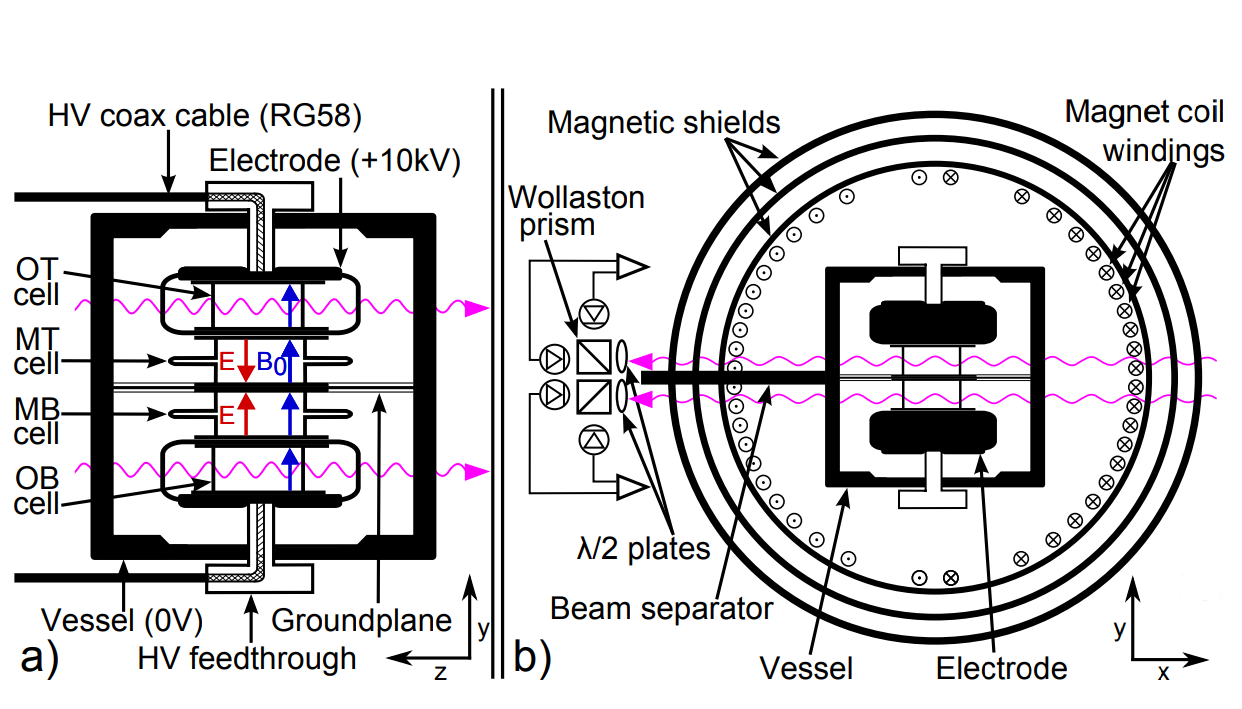
\includegraphics[width=0.75\textwidth]{199HgExperiment.png}
	\caption{ Schematic diagram of the $^{199}$ Hg EDM measurement presented by Graner, Chen, Lindahl and Heckel \cite{Graner2016}. a) Shows a YZ-plane cross-section of the experiment that illustrates the four cells used.  Two cells are located between the electrodes and two are are inside the electrodes. b) Shows the XY-plane cross-section of the experiment with the cylindrical magnetic shielding. The coils to produce a constant uniform $B_0$-field about which the magnetic moment precesses is also shown.}
		\label{fig:HgApp}
\end{figure}

The experiment is conducted with the apparatus depicted in Fig. \ref{fig:HgApp}. The apparatus  consists of four vapor cells containing $^{199}$Hg vapour, two cells are used as measurement cells and two are used as magnetometers. The cells are arranged in a stack at the Outer-Top (OT), Middle-Top (MT), Middle-Bottom (MB), and Outer Bottom (OB). The OT and OB vapor cells are located in a region with an E-field of zero and are used as magnetometers. The vapor cells in the middle positions have  E-fields with the same magnitude and opposing direction. 

The phase $\phi$ can be extracted from the decaying sinusoidal signal from the Faraday rotation, and is related to the Larmor frequency by measuring the asymmetry of the signal intensities
\begin{equation}\label{eq:wollaston}
    S(t) = \frac{I_S(t)-I_P(t)}{I_S(t)+I_P(t)} = \sin{ 2\theta }\approx 2\theta_0 sin{(\omega t + \phi)}e^{-t/\tau}.
\end{equation}%Wollaston separation and measuring of the S and P component of light
In Eq. \ref{eq:wollaston} the S and P components of light are required to be time averaged. This is done with a $\lambda/2$ wave plate so that the time averaged signal is equal. The components S and P are then detected separately by passing through a Wollaston prism. The signal $S(t)$ is approximately proportional to twice the angle of the decaying Faraday rotation of the probe laser as it passes through the Hg atoms. The decay constant is given by $\tau$. After fitting the two signal periods the phases of any two different cells is used to determine the frequency difference between cells. The beat signal $\mathcal{B}$(t) between any arbitrary cell pair $n$ and $m$ is the given by
\begin{equation}
    \mathcal{B}(t)=2\sin{\big(\Delta \omega_{mn}t_i+\Delta \phi_{mn} \big)} = \frac{S_m(t_i)S'_n(t_i)-S_n(t_i)S'}{N_m(t_i)N_n(t_i)}
\end{equation}
where
\begin{equation}
\begin{split}
       S'(t_i)=& S(t_{i+6})-S(t_{i-6}),\\
    N(t_i) =& \sqrt{S^2(t_i)-S(t_{i+6})S(t_{i-6})} = 4|\theta|e^{-t_i/\tau}, \; \textrm{and}\\
    S(t_{i\pm 6})=&\pm 2 \theta_0 \cos(\omega t + \phi)e^{-t_{i\pm 6}/\tau}.
\end{split}
\end{equation}

Here $t_{i\pm6}$ is the time that the signal is 1/4 of the wavelength along the signal. The 6 subscript is used since there are 24 points per wavelength measured. The dark frequency difference between two cells is $\Delta \omega^D_{mn} = \big( \Delta \phi^B_{mn}-\Delta \phi^A_{mn} \big)/\Delta t^D$. The frequency change related to the \gls{edm} change is defined as:
\begin{equation}
    \Delta \omega_{\textrm{EDM}^D} = \Delta \omega_{\textrm{MT-MB}}^D-k\Delta \omega_{\textrm{OT-OB}}^D.
\end{equation}
This frequency difference uses the comagnetometer frequency measurements along with a factor $k$. This statistical factor is tuned such that it reduces the variance in the data from a single day of running. 

\chapter{Current limits of EDMs}

The upper bounds of EDM measurements have been lowered over the last ~70 years as experiments reduce their statistical and systematical uncertainties in their \gls{edm} measurements of different atomic species and particles. Figure \ref{fig:EDMsearch} summarizes the uncertainties of the EDM measurements of the electron and neutron as well as atomic EDMs from Rd, Hg, and Xe.   

\begin{figure} [h!]
	\center
	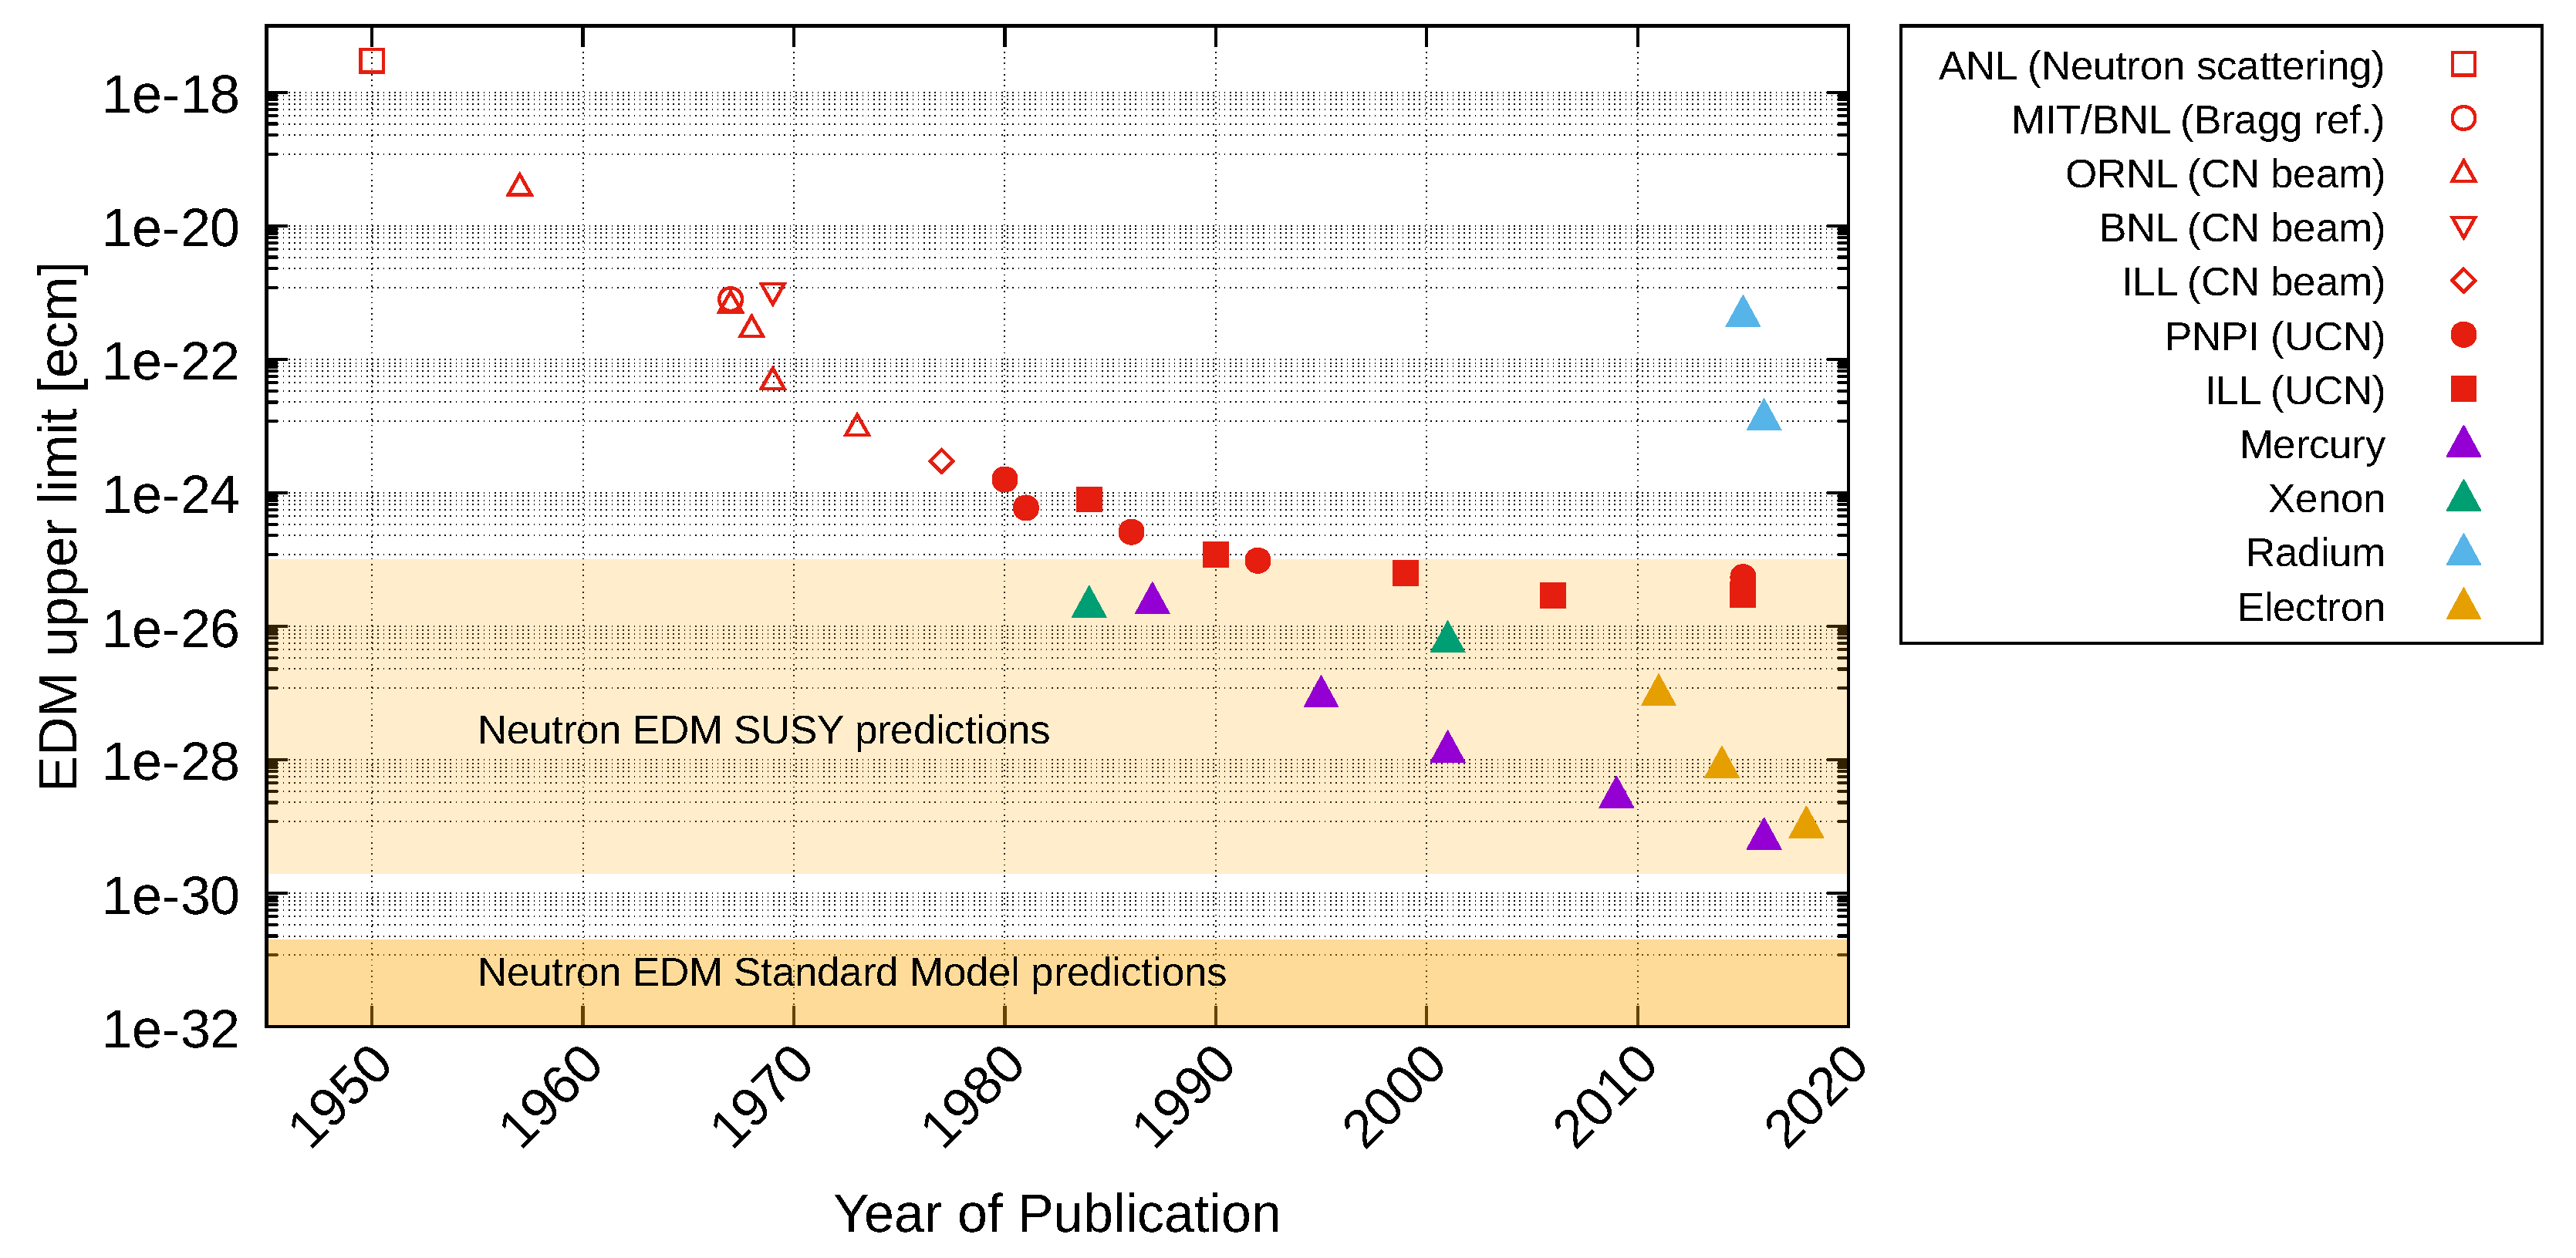
\includegraphics[width=.8\textwidth]{EDM-searches.png}
	\caption { The \gls{edm} measurements have been placing bounds that have been steadily going down over time,  as presented by Kuchler \cite{Kuchler}}.
		\label{fig:EDMsearch}
\end{figure}

The \gls{edm} predictions from beyond \gls{sm} physics are starting to be tested for the high energies interaction terms that contribute to EDMs at the TeV scale \cite{Chupp2015}. As the measured upper bound of $d_n$, $d_{^199\textrm{Hg}}$, and $d_{^199\textrm{Xe}}$ continue to be lowered from precision experiments, improved limits on beyond SM theories that have additional CP-violating physics are set. The search for EDMs play an important role probing new physics.

\clearpage

%
\addcontentsline{toc}{chapter}{Glossary}
\printnoidxglossaries
%\printglossary


%.tex method to make a references section
%\addcontentsline{toc}{chapter}{References}
\begin{thebibliography}{99}

\bibitem{Chupp2019}\href{https://journals.aps.org/rmp/abstract/10.1103/RevModPhys.91.015001}{T.E. Chupp, P. Fierlinger, M.J. Ramsey-Musolf, J.T. Singh, Reviews of Modern Physics \textbf{91} (2019) 015001.}

\bibitem{Pospelov2005}\href{https://www.sciencedirect.com/science/article/pii/S0003491605000539?via\%3Dihub}{M. Pospelov and A. Ritz, Annals of Physics \textbf{318}, 1 (2005): 119-169.  }

\bibitem{Engel2013} \href{https://www.sciencedirect.com/science/article/pii/S0146641013000227?via\%3Dihub}{ J. Engel, M.J. Ramsey-Musolf, U. Kolck, Progress in Particle and Nuclear Physics \textbf{71} (2013) 21-74.}

\bibitem{Sakharov} A. D. Sakharov, ZhETF Pis'ma 5, 1, (1967): 32-35.

\bibitem{Harris2007}\href{https://arxiv.org/pdf/0709.3100.pdf}{ P. G. Harris, arXiv:0709.3100, (2007).}

\bibitem{Flambaum}\href{https://journals.aps.org/pra/abstract/10.1103/PhysRevA.65.032113}{V. V. Flambaum and J. S. M. Ginges, Phys. Rev. A \textbf{65} (2002) 032113.}

\bibitem{Sushkov}\href{http://www.jetp.ac.ru/cgi-bin/e/index/e/60/5/p873?a=list}{O. P. Sushkov, V. V. Flambaum, and I. B. Khriplovich, Zh. Eksp. Teor. Fiz. \textbf{87} (1984).}


\bibitem{Helaine2014}\href{https://tel.archives-ouvertes.fr/tel-01063399/document}{V. H\'elaine, Ph. D. Thesis, Universit\'e de Caen Basse-Normandie (2014).}

\bibitem{Ramsey1980}\href{https://physicstoday.scitation.org/doi/10.1063/1.2914161}{N. F. Ramsey, Physics Today \textbf{33}, 7 (1980): 25-30.}
%change to Ramsey of update this reference

\bibitem{Golub} R. Golub, D. Richardson, and S. Lamoreaux, Ultra-cold neutrons, CRC Press, 1991. 

\bibitem{Norrgard2010}\href{https://journals.aps.org/pra/abstract/10.1103/PhysRevA.82.033408}{E. B. Norrgard, et al., Phys. Rev. A \textbf{82} (2010) 033408.}

\bibitem{Happer1984} \href{https://journals.aps.org/pra/abstract/10.1103/PhysRevA.29.3092}{W. Happer et al., Phys. Rev. A \textbf{29} (1984).}

\bibitem{Rosenberry2000} M. A. Rosenberry, Ph. D. Thesis, The University of Michigan (2000).

\bibitem{McFerran2014}\href{}{J. J. McFerran, et al., Phys. Rev. A \textbf{89} 4 (2014) 043432.}

\bibitem{Pendlebury2015} \href{https://journals.aps.org/prd/abstract/10.1103/PhysRevD.92.092003}{J. M. Pendlebury et al., Phys. Rev. D \textbf{92} (2015) 092003.}

\bibitem{Baker2006} \href{https://journals.aps.org/prl/abstract/10.1103/PhysRevLett.97.131801}{C. A. Baker et al., Phys. Rev. Lett. \textbf{97} (2006) 131801.}

\bibitem{Baker2014} \href{https://www.sciencedirect.com/science/article/pii/S0168900213013193}{C. A. Baker et al., Nucl. Instr. and Meth. Phys Res. A \textbf{736} 1 (2014).}

\bibitem{Rosenberry2001}\href{https://journals.aps.org/prl/abstract/10.1103/PhysRevLett.86.22}{M. A. Rosenberry and T. E. Chupp, Phys. Rev. Lett. \textbf{82}, 22 (2001).}

\bibitem{Graner2017}\href{https://journals.aps.org/prl/abstract/10.1103/PhysRevLett.119.119901}{B. Graner, Y. Chen, E. G. Lindahl, and B. R. Heckel, Phys. Rev. Lett. \textbf{119} (2017) 119901.}

\bibitem{Graner2016}\href{https://journals.aps.org/prl/abstract/10.1103/PhysRevLett.116.161601}{B. Graner, Y. Chen, E. G. Lindahl, and B. R. Heckel, Phys. Rev. Lett. \textbf{116} (2016) 161601.}

\bibitem{Griffith2009}\href{https://journals.aps.org/prl/abstract/10.1103/PhysRevLett.102.101601}{ W.C. Griffith, M.D. Swallows, T.H. Luftos, M.V. Romalis, B.R. Heckel, and E.N. Fortson, Phys. Rev. Lett. \textbf{102} (2009) 101601.}

\bibitem{Kuchler} \href{https://www.mdpi.com/2218-1997/5/2/56}{F. Kuchler, Universe, \textbf{5}, 2 (2019): 56.}
%drop the diagram in favour of chart that was presented during Can. Exam presentation and not worry about citation's quality 

\bibitem{Chupp2015} \href{https://journals.aps.org/prc/abstract/10.1103/PhysRevC.91.035502}{T.E. Chupp, M.J. Ramsey-Musolf, Phys. Rev. C \textbf{91} (2015) 035502.}

















\end{thebibliography}

\end{document}